% !TeX program = xelatex
% Build independently in this directory: xelatex defense_slides;
% bibtex defense_slides; xelatex defense_slides; xelatex defense_slides.
% English counterpart of ../Persian/defense_slides.tex, read in full with
% both bibliographies and the thesis geometry, method, results, conclusions.
% 30 main frames, approximately 27 minutes; four backups and references.
% Empirical evidence belongs to the joint SORA paper; no new experiments.
\documentclass[11pt,aspectratio=169,professionalfonts]{beamer}
\usetheme{Madrid}
\usecolortheme{whale}
\usepackage{amsmath,amssymb,booktabs,array,graphicx}
\usepackage{tikz}
\usetikzlibrary{arrows.meta,positioning}
\usepackage{appendixnumberbeamer}
\usepackage{fix-cm} % Scalable math fonts at caption and table sizes.
\usepackage{fontspec}
\setmainfont{TeX Gyre Termes}
\setsansfont{TeX Gyre Termes}
\setbeamerfont{normal text}{size=\fontsize{13}{17}}
\setbeamerfont{frametitle}{size=\fontsize{19}{23},series=\bfseries}
\setbeamerfont{block title}{size=\normalsize,series=\bfseries}
\setbeamerfont{caption}{size=\fontsize{10}{12}}
\setbeamerfont{footnote}{size=\fontsize{9}{11}}
\AtBeginEnvironment{frame}{\fontsize{13}{17}\selectfont}
\graphicspath{{./images/}}
\definecolor{sharifblue}{RGB}{0,51,102}
\definecolor{accent}{RGB}{0,121,140}
\setbeamercolor{structure}{fg=sharifblue}
\setbeamercolor{title}{fg=white,bg=sharifblue}
\setbeamercolor{frametitle}{fg=white,bg=sharifblue}
\setbeamercolor{palette primary}{fg=white,bg=sharifblue}
\setbeamercolor{palette secondary}{fg=white,bg=sharifblue!80}
\setbeamercolor{palette tertiary}{fg=white,bg=sharifblue!60}
\setbeamercolor{block title}{fg=white,bg=sharifblue}
\setbeamercolor{block body}{fg=black,bg=sharifblue!5}
\setbeamercolor{alerted text}{fg=accent}
\setbeamersize{text margin left=8mm,text margin right=8mm}
\setbeamertemplate{navigation symbols}{}
\setbeamertemplate{headline}{}
\setbeamertemplate{caption}{\raggedright\insertcaption\par}
\setbeamertemplate{itemize item}{\color{accent}\textbullet}
\setbeamertemplate{bibliography item}[text]
\setbeamertemplate{footline}{%
  \leavevmode\hbox{%
    \begin{beamercolorbox}[wd=.27\paperwidth,ht=3ex,dp=2ex,center]{author in head/foot}
      \fontsize{9}{10}\selectfont Farzan Rahmani
    \end{beamercolorbox}%
    \begin{beamercolorbox}[wd=.57\paperwidth,ht=3ex,dp=2ex,center]{title in head/foot}
      \fontsize{9}{10}\selectfont MSc Defense | Fast Adversarial Training
    \end{beamercolorbox}%
    \begin{beamercolorbox}[wd=.16\paperwidth,ht=3ex,dp=2ex,center]{date in head/foot}
      \fontsize{9}{10}\selectfont\insertframenumber\,/\,\inserttotalframenumber
    \end{beamercolorbox}}}
% Provenance: original seminar institutional logo; branding, not research evidence.
\logo{
\includegraphics[height=5mm]{logo.pdf}\hspace{1mm}}
\setbeameroption{hide notes} % Change to show notes for presenter output.
\newcommand{\src}[1]{\par\vspace{1mm}{\fontsize{9}{11}\selectfont\color{sharifblue}#1\par}}
\newcommand{\takeaway}[1]{\begin{block}{Takeaway}#1\end{block}}
\newcommand{\sora}{SORA}
\newcommand{\pa}{PertAlign}
\DeclareMathOperator{\sign}{sign}
\title{Predicting Catastrophic Overfitting in Fast Adversarial Training}
\author{Farzan Rahmani}
\institute{Sharif University of Technology\\Department of Computer Engineering}
\date{} % No defense date or committee was supplied.
\hypersetup{pdftitle={Predicting Catastrophic Overfitting in Fast Adversarial Training},
  pdfauthor={Farzan Rahmani},pdfsubject={MSc Defense; SORA}}
\pdfstringdefDisableCommands{\def\translate#1{#1}}

\begin{document}

% MAIN 01 | 0:40
\begin{frame}[plain]
\centering
% Provenance: original seminar institutional logo; branding only.

\includegraphics[height=13mm]{logo.pdf}\par
{\fontsize{12}{16}\selectfont Sharif University of Technology | Department of Computer Engineering\par}
{\fontsize{12}{16}\selectfont MSc Thesis Defense in Computer Engineering: Artificial Intelligence and Robotics\par}
\vspace{4mm}
\begin{beamercolorbox}[wd=\textwidth,sep=3mm,center,rounded=true]{title}
{\fontsize{21}{26}\selectfont\bfseries Predicting Catastrophic Overfitting\\in Fast Adversarial Training\par}
\end{beamercolorbox}
\vspace{4mm}
Farzan Rahmani \quad | \quad Student ID: 403210725\par
Supervisor: Dr. Mohammad Hossein Rohban
\note{Target duration: approximately 27 minutes. The title follows the supplied initial proposal. The goal is to anticipate failure of single-step training at low cost and connect that warning to step-size correction. In English, adversarial is used consistently for the corresponding terminology in the Persian thesis.}
\end{frame}

% MAIN 02 | 0:40
\begin{frame}{Defense Roadmap: From Failure to Step-Size Control}
\begin{enumerate}
\item Problem: why can high single-step accuracy be misleading?
\item Analysis and method: loss geometry, \pa{}, and the \sora{} controller.
\item Evidence: robustness, transfer of settings, computational cost, and limits.
\end{enumerate}
\src{Scientific basis: the joint \sora{} paper at ICML 2026 \cite{sora2026}; thesis Chapters 1--7 and the appendix.}
\note{The joint paper's authors, in order, are Mazdak Teymourian, Ramtin Moslemi, Farzan Rahmani, and Mohammad Hossein Rohban. All empirical numbers and plots are from that paper; no new experiments were run in preparing the thesis. Allocate about 6 minutes to the problem, 13 to analysis and method, and 8 to evidence and conclusions.}
\end{frame}

% MAIN 03 | 0:50
\begin{frame}{Practical Question and Threat Model}
\begin{itemize}
\item Detect and correct a failing single-step approximation using information already available during training.
\item An untargeted, white-box attacker increases the image-classification loss.
\item The metric is empirical accuracy under strong attacks, not a mathematical robustness certificate.
\end{itemize}
\[
\Delta_\infty(x,\epsilon)=\{\delta:\|\delta\|_\infty\leq\epsilon,
\quad x+\delta\in[0,1]^d\}
\]
\src{Threat model and evaluation: \cite{madry2018towards,croce2020reliable}.}
\note{The perturbation budget is measured in pixel space before normalization. The threat set combines an infinity-norm bound with valid pixel values. The claim concerns robustness to this numerical threat model.}
\end{frame}

% MAIN 04 | 0:50
\begin{frame}{Adversarial Training: Two Coupled Problems}
\[
\min_\theta\;\mathbb E_{(x,y)\sim\mathcal D}
\left[\max_{\delta\in\Delta_\infty(x,\epsilon)}
\mathcal L(f_\theta(x+\delta),y)\right]
\]
\begin{itemize}
\item Inner problem: find a high-loss example for the current model.
\item Outer problem: update the weights using that example.
\item Fast training reduces the cost of the inner solve; its approximation quality needs monitoring.
\end{itemize}
\src{Formulation: \cite{madry2018towards}; fast training: \cite{wong2020fast}.}
\note{Write the loss as ell of the input when the label and parameters are fixed. Progress on the outer problem is meaningful only to the extent that the inner solver still finds useful adversarial examples.}
\end{frame}

% MAIN 05 | 1:00
\begin{frame}{One Gradient Versus Repeated Direction Updates}
\textbf{Fast Gradient Sign Method (FGSM): a first-order approximation}
\[
g=\nabla_x\ell(x),\qquad
x_{\mathrm{FGSM}}=\Pi_{[0,1]^d}(x+\epsilon\sign(g))
\]
\textbf{Projected Gradient Descent (PGD): a multi-step attack}
\[
\delta^{t+1}=\Pi_{\Delta_\infty(x,\epsilon)}
\left(\delta^t+a\sign\bigl(\nabla_x\ell(x+\delta^t)\bigr)\right)
\]
\begin{itemize}
\item FGSM keeps the initial direction; PGD observes changes in direction.
\item The perturbation budget $\epsilon$ and step size $a$ are different quantities.
\end{itemize}
\src{FGSM: \cite{goodfellow2015explaining}; PGD: \cite{madry2018towards}.}
\note{Although called projected gradient descent in the literature, the attack here ascends the classification loss. Its projection enforces the evaluation threat set. The simple FGSM expression shown starts from the clean input.}
\end{frame}

% MAIN 06 | 0:45
\begin{frame}{Catastrophic Overfitting: Apparent Solver Success}
\begin{itemize}
\item Accuracy under a multi-step attack collapses over a short interval.
\item Accuracy under the single-step training attack may remain high.
\item Low loss at the attack endpoint does not bound the maximum loss nearby.
\end{itemize}
\takeaway{Assess the training-example generator itself: evaluation with the training attack alone is insufficient.}
\src{Definition and analysis: \cite{wong2020fast,andriushchenko2020understanding}.}
\note{This phenomenon differs from gradual robust generalization degradation. A model can repair the points reached by a weak generator while high-loss points remain along the path between them.}
\end{frame}

% MAIN 07 | 1:10
\begin{frame}{What Do Previous Methods Change?}
% Provenance: newly composed qualitative table from SORA Section 2 and the
% thesis literature review; not an original paper/seminar table or experiment.
\begin{table}
\centering\fontsize{11}{14}\selectfont
\renewcommand{\arraystretch}{1.25}
\begin{tabular}{>{\raggedright\arraybackslash}p{.20\linewidth}>{\raggedright\arraybackslash}p{.29\linewidth}>{\raggedright\arraybackslash}p{.38\linewidth}}
\toprule
Family & Examples & Mechanism and open question \\
\midrule
Perturbation diversity & FGSM-RS, N-FGSM & Vary starts and amplitudes; do settings transfer? \\
Regularization & GradAlign, NuAT, ELLE & Control geometry; at what computational cost? \\
Abnormal examples & AAER & Control loss decrease; how early is the signal? \\
Adaptive steps & ATAS & Use gradient magnitude; what about curvature? \\
\bottomrule
\end{tabular}
\caption{New synthesis of the review in \sora{} Section 2 \cite{sora2026}; this table does not appear in the paper or seminar.}
\end{table}
\src{Methods: \cite{dejorge2022make,andriushchenko2020understanding,sriramanan2021towards,rocamora2024efficient,lin2023eliminating,huang2023fast}.}
\note{These families organize the literature by the part of fast training they modify. The table is a qualitative synthesis, not a new numerical comparison. The open questions motivate monitoring geometry with gradients already computed during training.}
\end{frame}

% MAIN 08 | 0:55
\begin{frame}{Geometry: One Step Can Skip a Vulnerable Region}
% Provenance: local paper_geometry.pdf, published SORA Figure 1;
% original paper figure reproduced unchanged, not seminar or new evidence.
\begin{figure}
\centering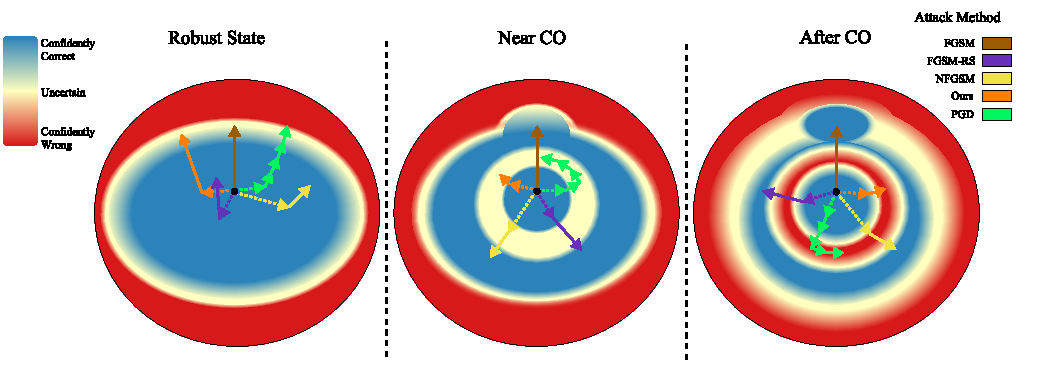
\includegraphics[width=\linewidth,height=.50\paperheight,keepaspectratio]{paper_geometry.pdf}
\caption{Decision-boundary distortion and loss-surface evolution; reproduced from \sora{} Figure 1 \cite{sora2026}.}
\end{figure}
\centering A low-loss endpoint can hide high-loss points along the path.
\note{Explain from left to right: the initial geometry, changes before collapse, and then single-step failure. This is the paper's interpretation of a mechanism, not a universal theorem about all networks.}
\end{frame}

% MAIN 09 | 0:55
\begin{frame}{Epsilon Overfitting: Sensitivity to Perturbation Size}
% Provenance: local paper_epsilon.pdf, published SORA Figure 2;
% original paper sweep, no new measurements or seminar results.
\begin{figure}
\centering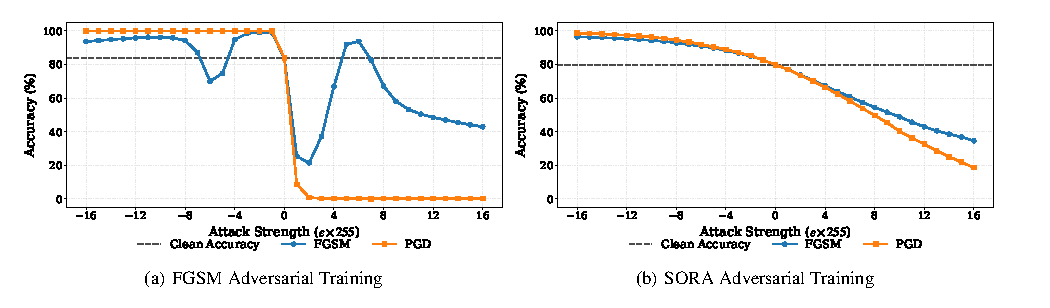
\includegraphics[width=\linewidth,height=.48\paperheight,keepaspectratio]{paper_epsilon.pdf}
\caption{Accuracy across attack sizes; reproduced from \sora{} Figure 2 \cite{sora2026}.}
\end{figure}
\begin{itemize}
\item Learning at particular sizes does not protect the whole neighborhood.
\item Negative axis values reverse the direction; the threat radius is not negative.
\end{itemize}
\note{Nonmonotonicity concerns the response to an approximate attack. The exact maximum loss on nested sets cannot decrease as the radius grows. Epsilon overfitting explains part of the phenomenon; it is not a proved necessary and sufficient condition for every collapse.}
\end{frame}

% MAIN 10 | 0:45
\begin{frame}{Abnormal Adversarial Examples: Overshooting a Peak}
\[
z=x+\eta,\qquad \ell(z+\delta)<\ell(z)
\]
\begin{itemize}
\item The attack aims to increase loss, yet reduces it at the endpoint.
\item An AAE is abnormal in terms of loss, not necessarily label correctness.
\item The gradient direction can change before this loss decrease appears.
\end{itemize}
\takeaway{Comparing two gradients can provide information earlier than comparing two losses.}
\src{AAE definition: \cite{lin2023eliminating}; motivation for geometric monitoring: \cite{sora2026}.}
\note{Use the noisy start z as the reference in this expression. An abnormal endpoint need not be classified correctly. Conversely, a small loss increase does not establish that the attack is strong.}
\end{frame}

% MAIN 11 | 0:55
\begin{frame}{Perturbation Alignment: Two Available Gradients}
\[
g=\nabla\ell(z),\quad g'=\nabla\ell(z+\delta),\qquad
P=\frac{g^{\mathsf T}g'}{\|g\|_2\|g'\|_2}
\]
\begin{itemize}
\item \pa{} compares gradient directions at the start and end of the attack.
\item The first gradient constructs the attack; the second accompanies backpropagation on the adversarial example.
\item A value near one means directional agreement, not necessarily low curvature.
\end{itemize}
\src{Equation 2, p.\ 5 of \sora{} \cite{sora2026}; defined for nonzero gradients.}
\note{Obtaining the input derivative in the second pass does not require a new attack loop. Norms and dot products have a limited but nonzero cost. A reproduction must specify protection against zero denominators. In implementation, the second gradient is with respect to the final clipped input itself.}
\end{frame}

% MAIN 12 | 1:00
\begin{frame}{Warning Evidence: About 50 Batches}
% Provenance: local paper_pertalign.pdf, SORA Figure 3; timing read using
% paper pp.44--46 and thesis results, not a calibrated predictor study.
\begin{figure}
\centering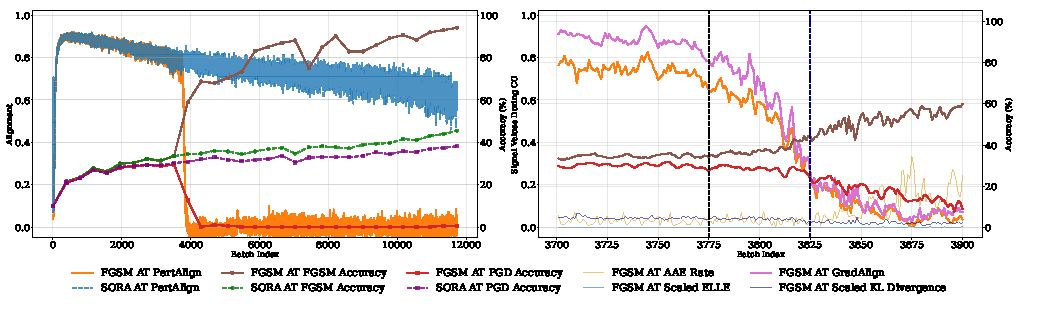
\includegraphics[width=\linewidth,height=.39\paperheight,keepaspectratio]{paper_pertalign.pdf}
\caption{Alignment falls before accuracies separate; reproduced from \sora{} Figure 3 \cite{sora2026}.}
\end{figure}
\begin{itemize}
\item One FGSM trajectory: decline around batch $3775$; clear separation around $3825$.
\item This is not an average or guaranteed lead time; no threshold or false-alarm rate is reported.
\end{itemize}
\note{These approximate readings come from the plots discussed on pages 44--46. GradAlign also responds early, and an appropriately transformed ELLE metric can change at a similar point. The claimed advantage combines response timing with reuse of existing gradients. Do not convert 50 batches into epochs or seconds without the trajectory's specifications.}
\end{frame}

% MAIN 13 | 1:05
\begin{frame}{Geometric Relation: Projected Hessian Action}
For $g\ne0$, a fixed direction $v$, and a small step $\alpha$:
\[
H=\nabla^2\ell(z),\qquad
Q_g=I-\frac{gg^{\mathsf T}}{\|g\|_2^2}
\]
\[
1-P=\frac{\alpha^2}{2\|g\|_2^2}\|Q_gHv\|_2^2+O(\alpha^3)
\]
\begin{itemize}
\item Assumptions: local smoothness and a locally Lipschitz Hessian; hold the direction fixed in the expansion.
\item $P\approx1$ does not imply a small $\|H\|$: parallel gradient changes are invisible.
\end{itemize}
\src{Projected reformulation in the thesis geometry chapter, based on Appendix A of \sora{} \cite{sora2026}.}
\note{If needed, give the example H equals M times the identity and v equals g. The endpoint gradient is only rescaled, so the cosine remains one even for large M. The expansion also applies to a fixed sign direction, but the special formula for direction g must not be transferred unchanged to its sign.}
\end{frame}

% MAIN 14 | 1:10
\begin{frame}{Exact Theory: Scalar Optimum of a Quadratic Model}
\[
p=\sign(g),\quad q(a)=\ell(z)+ba+\tfrac12ca^2,
\quad b=\|g\|_1>0,\ c=p^{\mathsf T}Hp
\]
\[
\underset{0\leq a\leq A}{\arg\max}\;q(a)=
\begin{cases}
\min\{A,-b/c\},&c<0,\\
A,&c\geq0.
\end{cases}
\]
\begin{itemize}
\item In a concave direction, moving beyond the vertex reduces loss.
\item This solves the scalar model exactly; the real loss need not be quadratic.
\end{itemize}
\src{Thesis method derivation, based on the second-order analysis in \sora{} \cite{sora2026}.}
\note{For nonnegative c and positive b, the derivative is positive on the nonnegative half-line, so the endpoint is optimal. A positive vertex occurs only for negative c. Keep the nonzero-gradient assumption: the theoretical ratios are undefined at a zero gradient.}
\end{frame}

% MAIN 15 | 1:00
\begin{frame}{Curvature Information from the Same Probe Step}
In a quadratic model, without clipping, for a scalar probe $a_{\mathrm{probe}}>0$:
\[
g_{\mathrm{probe}}=g+a_{\mathrm{probe}}Hp,\qquad
r=\frac{p^{\mathsf T}g_{\mathrm{probe}}}{\|g\|_1}
=1+\frac{a_{\mathrm{probe}}c}{b}
\]
\[
r<1\quad\Longrightarrow\quad
a_{\mathrm{quad}}=\min\left\{A,\frac{a_{\mathrm{probe}}}{1-r}\right\}
\]
\begin{itemize}
\item The numerator is the actual step used to measure the second gradient.
\item The ratio $r$ is not the \pa{} cosine: gradient magnitude also matters.
\end{itemize}
\src{Exact reformulation in the thesis method chapter from the \sora{} derivation \cite{sora2026}.}
\note{For r at least one the constrained optimum is A. The probe identity depends on the same scalar step appearing in the gradient measurement and in the numerator; it does not authorize replacing that step by an arbitrary constant.}
\end{frame}

% MAIN 16 | 1:00
\begin{frame}{Practical Rule: Quadratic-Inspired Amplitude Control}
\[
F(u)=\begin{cases}
\min\!\left\{\alpha_{\max},\dfrac{\alpha_0}{1-u}\right\},&u<1,\\
\alpha_{\max},&u\geq1,
\end{cases}
\qquad a_j\sim\mathcal U(0,A_i)
\]
\begin{itemize}
\item $u$ is an exponential moving average of the ratio; $A_i$ caps the componentwise step distribution.
\item Replacing the probe step by $\alpha_0$ changes the previous exact identity.
\item Componentwise randomness and use of past batches are further practical choices.
\end{itemize}
\src{\sora{} Algorithm 1 \cite{sora2026}: $\alpha_0=0.02$, $\beta=0.05$, $\alpha_{\max}=2\epsilon$.}
\note{Call this an adaptive cap rather than an optimal step for each example. With componentwise amplitudes, the second gradient depends on H times diag(a) times p and need not satisfy the scalar-probe relation. Empirical success does not guarantee global optimality.}
\end{frame}

% MAIN 17 | 0:40
\begin{frame}{Why Can Step-Size Correction Help?}
% Provenance: local paper_recovery.pdf, SORA Figure 4; original conceptual
% illustration, not a new recovery experiment or a universal guarantee.
\begin{figure}
\centering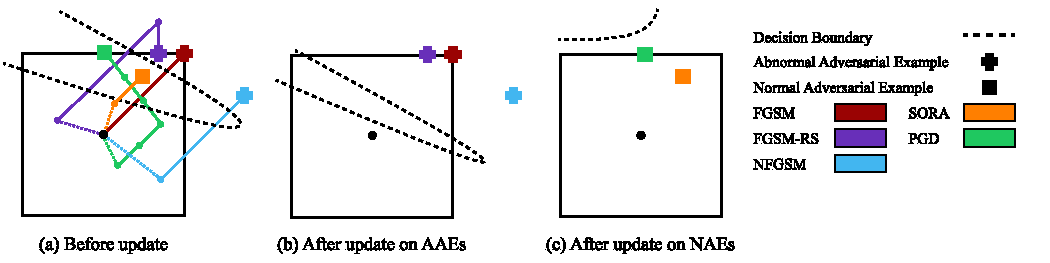
\includegraphics[width=\linewidth,height=.50\paperheight,keepaspectratio]{paper_recovery.pdf}
\caption{Geometric interpretation of step-size correction; reproduced from \sora{} Figure 4 \cite{sora2026}.}
\end{figure}
\centering Reaching high-loss points can redirect training toward the vulnerable region.
\note{The figure explains a mechanism; it does not guarantee recovery after every collapse. Amplitude control tries to avoid skipping the high-loss region in a single long step.}
\end{frame}

% MAIN 18 | 0:55
\begin{frame}{The SORA Pipeline: Reusing Two Passes}
% Provenance: newly composed flow diagram from SORA Algorithm 1 p.6;
% this exact diagram is not an original paper or seminar figure.
\begin{figure}
\centering
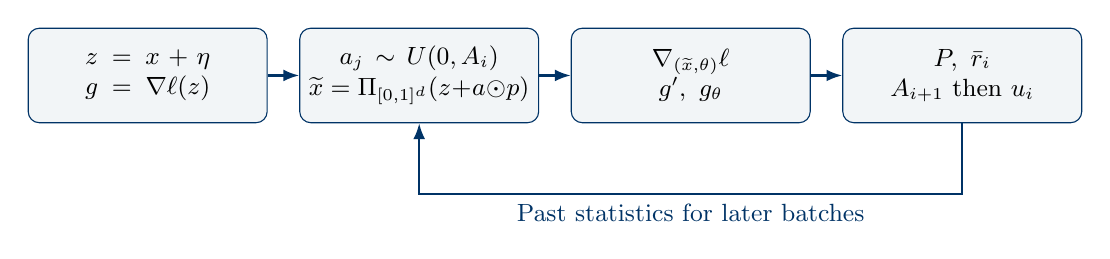
\begin{tikzpicture}[node distance=4mm,
 stage/.style={draw=sharifblue,rounded corners,fill=sharifblue!5,
   minimum height=12mm,text width=28mm,align=center,font=\small},
 flow/.style={-{Latex[length=2mm]},thick,sharifblue}]
\node[stage] (start) {$z=x+\eta$\\$g=\nabla\ell(z)$};
\node[stage,right=of start] (attack) {$a_j\sim U(0,A_i)$\\$\widetilde x=\Pi_{[0,1]^d}(z+a\odot p)$};
\node[stage,right=of attack] (train) {$\nabla_{(\widetilde x,\theta)}\ell$\\$g',\ g_\theta$};
\node[stage,right=of train] (control) {$P,\ \bar r_i$\\$A_{i+1}$ then $u_i$};
\draw[flow] (start)--(attack);
\draw[flow] (attack)--(train);
\draw[flow] (train)--(control);
\draw[flow] (control.south)--++(0,-9mm)-|node[pos=.25,below,font=\small]
  {Past statistics for later batches} (attack.south);
\end{tikzpicture}
\caption{New diagram of Algorithm 1 \cite{sora2026}; this diagram does not appear in the original paper or seminar.}
\end{figure}
\begin{itemize}
\item The second pass yields both the weight derivative and endpoint input gradient.
\item \pa{} monitors training; the ratio $r$ controls the step cap.
\end{itemize}
\note{Read the diagram from left to right, then follow the feedback arrow. Use stored input gradients for monitoring and control; no extra iterative attack is needed. The next slide makes the printed algorithm's ordering and delay explicit.}
\end{frame}

% MAIN 19 | 1:10
\begin{frame}{Pseudocode and the Printed Order's Extra Delay}
% Provenance: newly composed compact English restatement of SORA Algorithm 1,
% preserving line 11 before line 12. Explicit A1 initialization and batch
% reduction follow thesis conventions, not fully specified printed details.
\begingroup\fontsize{12}{15}\selectfont
\begin{enumerate}
\item Initialize $u_0=0.99$, $A_1=F(u_0)$; for each batch draw $\eta\sim U([-\epsilon,\epsilon]^d)$.
\item $g=\nabla\ell(x+\eta)$, $p=\sign(g)$; detach the attack direction.
\item Draw $a_j\sim U(0,A_i)$; form $\widetilde x=\Pi_{[0,1]^d}(x+\eta+a\odot p)$.
\item Obtain $(g',g_\theta)$; update weights; compute $\bar r_i$ by averaging per-example ratios.
\end{enumerate}\endgroup
\[
\boxed{A_{i+1}=F(u_{i-1})}\quad\text{then}\quad
u_i=(1-\beta)u_{i-1}+\beta\bar r_i
\]
\textbf{Batch $i$'s observation can first affect the cap at batch $i+2$.}
\src{Algorithm 1, p.\ 6 \cite{sora2026}; $A_1$ initialization and mean of ratios are explicit thesis method conventions.}
\note{The next-step line precedes the exponential-average line. This ordering has been preserved. Averaging per-example ratios differs from a ratio of sums; the paper does not specify the reduction. This explicit delay exists in addition to the temporal memory of the exponential average.}
\end{frame}

% MAIN 20 | 1:00
\begin{frame}{Training Domain and Evaluation Threat Ball Differ}
\[
\widetilde x=\Pi_{[0,1]^d}(x+\eta+a\odot p),\qquad
\|\eta+a\odot p\|_\infty\leq\epsilon+\alpha_{\max}=3\epsilon
\]
\begin{itemize}
\item Training: clip pixels to $[0,1]$ only; no projection onto the $\epsilon$-ball.
\item $3\epsilon$ bounds the raw perturbation; it is not every example's fixed size.
\item Evaluation: the $\epsilon$-ball and pixel domain; usually $8/255$, but $3/255$ for TissueMNIST.
\end{itemize}
\src{Algorithm 1 and Appendix D, p.\ 31 of \sora{} \cite{sora2026}.}
\note{In the original pseudocode, the first-gradient point x plus noise is also not clipped before evaluation. Adding that clipping or projecting onto the epsilon-ball changes the method. Interpret budgets in pixel space before normalization.}
\end{frame}

% MAIN 21 | 0:45
\begin{frame}{Adaptive Behavior Differs Across Two Datasets}
% Provenance: local paper_stepsize.pdf, SORA Figure 5; original published
% monitoring curves, not a new experiment or an exact-optimum trajectory.
\begin{figure}
\centering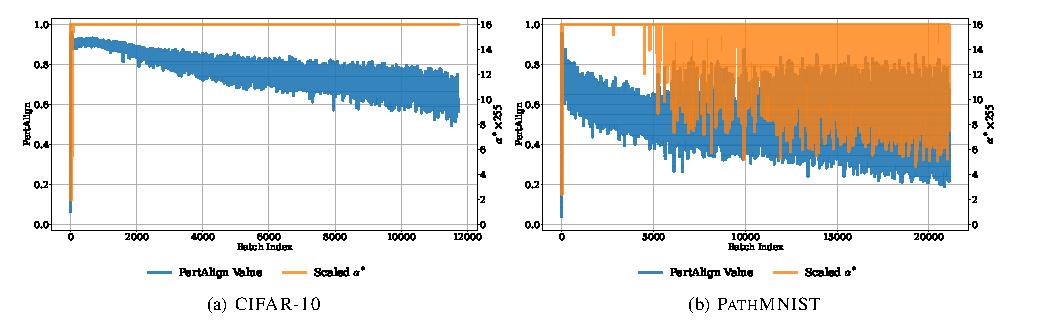
\includegraphics[width=\linewidth,height=.50\paperheight,keepaspectratio]{paper_stepsize.pdf}
\caption{Alignment and step cap; reproduced from \sora{} Figure 5 \cite{sora2026}.}
\end{figure}
\centering The cap is often active on CIFAR-10; step reductions are more frequent on PathMNIST.
\note{The plotted practical cap is not the exact quadratic optimum for every example. Different controller behavior across datasets is consistent with adaptation to their loss geometry, but does not prove an accurate curvature estimate in each batch.}
\end{frame}

% MAIN 22 | 0:55
\begin{frame}{Training Settings and Evaluation Scope}
\begin{itemize}
\item Datasets: CIFAR-10/100, TinyImageNet, ImageNet-100, PathMNIST, and TissueMNIST.
\item Architectures: PreActResNet-18, ResNet-18, WRN-28-10, and SENet-18; models are trained separately.
\item SGD: momentum $0.9$, weight decay $5\!\times\!10^{-4}$; cyclic learning rate for natural images, cosine for medical images.
\end{itemize}
\takeaway{``Fixed settings'' means a shared final parameter set after limited tuning; data preparation and all training details are not identical.}
\src{Section 6 and Appendices D, E, M.3, pp.\ 30--34 and 60 of \sora{} \cite{sora2026}.}
\note{Generalization here means transfer of settings across separately trained models, not testing a CIFAR model on medical images. Three seeds are reported for most experiments; ImageNet-100 has only one run. Data augmentation differs by dataset.}
\end{frame}

% MAIN 23 | 1:00
\begin{frame}{Main Results on Two Difficult Problems}
% Provenance: exact selected entries of SORA main Table 1 p.9;
% original table content with English headings, no new run or mixed reports.
\begin{table}
\centering\fontsize{12}{17}\selectfont\renewcommand{\arraystretch}{1.3}
\begin{tabular}{lrrrr}
\toprule
&\multicolumn{2}{c}{PathMNIST}&\multicolumn{2}{c}{ImageNet-100}\\
Method&Clean&AA&Clean&AA\\
\midrule
FGSM&46.06&0.42&15.94&0.00\\
N-FGSM&74.89&1.65&49.40&15.52\\
AAER&83.54&2.48&48.26&17.18\\
\bfseries SORA&\bfseries85.93&\bfseries32.91&\bfseries57.26&\bfseries18.56\\
\bottomrule
\end{tabular}
\caption{Selected data from Table 1, p.\ 9 \cite{sora2026}; PreActResNet-18, $\epsilon=8/255$; all values are percentages.}
\end{table}
\centering AA gains over N-FGSM: $31.26$ and $3.04$ percentage points, respectively.
\note{Read Table 1 independently. The ImageNet result is from one run; the 1.38 percentage-point difference from AAER cannot be called statistically significant. No ablation values or aggregate appendix results have been inserted here.}
\end{frame}

% MAIN 24 | 0:55
\begin{frame}{Transfer of Settings: Relative Performance Overview}
% Provenance: local paper_generalization.pdf, SORA Figure 6 p.8;
% normalization described p.47; original paper figure, no new aggregation.
\begin{figure}
\centering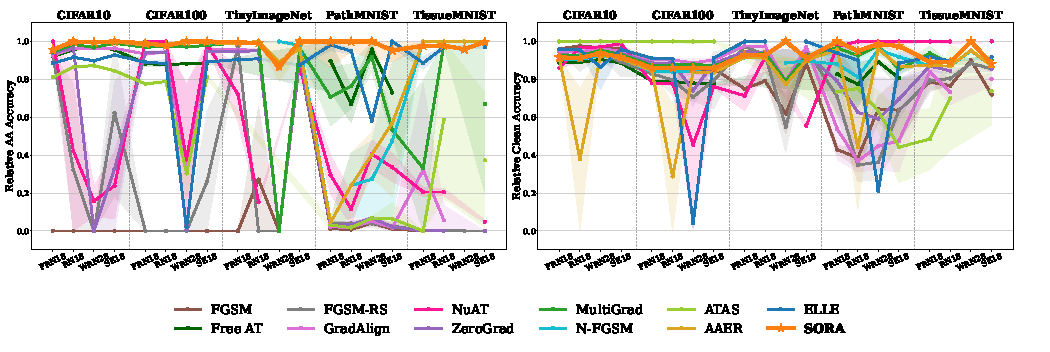
\includegraphics[width=\linewidth,height=.49\paperheight,keepaspectratio]{paper_generalization.pdf}
\caption{Reproduced from Figure 6, p.\ 8 \cite{sora2026}; normalized by each problem's best value, as described on p.\ 47.}
\end{figure}
\begin{itemize}
\item A value near one means proximity to the best result in that column.
\item This view hides absolute values and the size of small differences.
\end{itemize}
\note{The best clean and best adversarial accuracies may belong to different methods. The plot provides evidence about transferring the final settings; it does not establish superiority in every cell of the detailed tables.}
\end{frame}

% MAIN 25 | 0:55
\begin{frame}{Detailed Tables: No Method Wins Every Column}
% Provenance: newly composed selected central values from SORA Tables 20
% p.48, 24 p.50, 30 p.53; not an original paper/seminar table. +/- omitted.
\begin{table}
\centering\fontsize{12}{15}\selectfont\renewcommand{\arraystretch}{1.1}
\begin{tabular}{llrrr}
\toprule
Dataset / model & Method & Clean & PGD-10 & AA\\
\midrule
CIFAR-10 / PreAct-18 & N-FGSM &79.05&48.73&43.95\\
& SORA &79.90&48.64&43.83\\
CIFAR-100 / PreAct-18 & N-FGSM &53.43&26.25&21.75\\
& SORA &54.74&26.12&21.56\\
TinyImageNet / WRN-28-10 & N-FGSM &48.47&21.21&\bfseries16.58\\
& SORA &54.59&18.73&14.31\\
\bottomrule
\end{tabular}
\caption{New arrangement from Tables 20, 24, and 30, pp.\ 48, 50, and 53 \cite{sora2026}; central percentage values only, omitting $\pm$; not an original paper table.}
\end{table}
\centering Interpretation: a clean--robust--cost tradeoff; rankings depend on the problem.
\note{Keep the TinyImageNet WideResNet counterexample visible: N-FGSM has AA accuracy 16.58 versus SORA's 14.31, while SORA has higher clean accuracy. Even on the two CIFAR examples, SORA does not have the highest AA value.}
\end{frame}

% MAIN 26 | 0:55
\begin{frame}{Component Ablation: A Separate PGD-10 Report}
% Provenance: exact SORA main Table 2 p.9, PathMNIST/PreActResNet-18;
% original ablation content, not Table 1 AA values or new experiments.
\begin{table}
\centering\fontsize{12}{17}\selectfont\renewcommand{\arraystretch}{1.3}
\begin{tabular}{lrrr}
\toprule
Setting & Clean & FGSM & PGD-10\\
\midrule
SORA (baseline)&84.69&57.51&45.56\\
Without random sampling&85.67&58.89&45.35\\
Clamping step size&86.82&52.02&34.08\\
Without adaptive step size&89.93&28.30&17.23\\
\bottomrule
\end{tabular}
\caption{Table 2, p.\ 9 \cite{sora2026}; PathMNIST/PreActResNet-18, percentages; independent of the main AA report.}
\end{table}
\centering Removing adaptation causes a large drop; the $0.21$-point sampling drop alone does not establish statistical significance.
\note{The last row is called Without Optimal Step-Size in the paper; here it is described as without adaptive step size, not as a new claim of exact algorithmic optimality. The baseline clean value 84.69 and PGD-10 value 45.56 belong to this experiment. The table does not specify uncertainty for this comparison.}
\end{frame}

% MAIN 27 | 0:55
\begin{frame}{Efficiency: Time and Memory in One Setting}
% Provenance: local paper_efficiency.pdf, SORA Figure 7 p.8;
% protocol p.59: PathMNIST/PreAct-18, 30 epochs, RTX 4090, training loop only.
\begin{figure}
\centering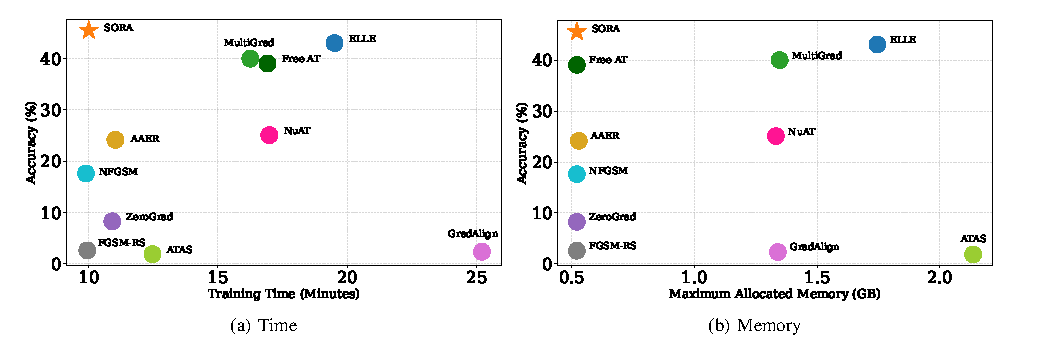
\includegraphics[width=\linewidth,height=.54\paperheight,keepaspectratio]{paper_efficiency.pdf}
\caption{Reproduced from Figure 7, p.\ 8 \cite{sora2026}; PathMNIST/PreActResNet-18, 30 epochs, RTX 4090; accuracy measured with PGD-10.}
\end{figure}
\note{Table 19 on page 48 gives SORA two forward and two backward passes, versus eleven of each for PGD-10. The pass ratio is not a measured speedup. Page 59 states that figure timing covers only the training loop, excluding saving, loading, and hyperparameter search. Do not extract new exact timing numbers from the plot. Dot products and gradient storage are not free. The missing ATAS result on TinyImageNet is due to memory limitations and must not be read as zero accuracy.}
\end{frame}

% MAIN 28 | 0:55
\begin{frame}{Evidence Limits and Defensible Claims}
\begin{itemize}
\item Warning: an observed temporal lead, without a calibrated predictor or false-alarm rate.
\item Theory: local and direction dependent; randomization, clipping, and delay depart from the exact model.
\item Evaluation: ImageNet-100 has one run; full attack details and relationships between some reports remain unclear.
\end{itemize}
\src{Thesis results, conclusions, and technical appendix; \sora{} Appendices J and M \cite{sora2026}.}
\note{Main-text and appendix numbers have not been corrected or merged. The medical results concern classification under numerical perturbations and do not establish clinical safety. Multi-step training may still provide higher robustness.}
\end{frame}

% MAIN 29 | 0:50
\begin{frame}{Contributions: Connecting Geometry to Training Control}
\begin{enumerate}
\item Epsilon-overfitting interpretation: cover diverse perturbation sizes and directions.
\item \pa{}: monitor gradient-direction changes using existing computation, with a local geometric interpretation.
\item \sora{}: control the step-distribution cap using two gradients; a competitive tradeoff within the evaluated scope.
\end{enumerate}
\src{Contributions of the joint research \cite{sora2026}; this defense presents the documented narrative and analysis of the completed thesis chapters.}
\note{Attribute these contributions to the joint paper. Author order is not evidence that a specific component belongs to one individual. The central result is the possibility of using geometry already available during training at low cost.}
\end{frame}

% MAIN 30 | 0:50
\begin{frame}{Future Work: Toward a Measurable Predictor}
\begin{itemize}
\item Define collapse independently, choose a validation threshold, and measure false alarms and lead time across multiple runs.
\item Study per-example or group control for imbalanced datasets; weigh gains against variance and cost.
\item Separate amplitude, diversity, and adaptation under matched computational budgets and training domains.
\end{itemize}
\takeaway{Two existing gradients can support both warning and step-size correction; independent robustness evaluation remains essential.}
\src{Directions proposed in the thesis conclusions; limitations of the joint study \cite{sora2026}.}
\note{These are future research directions, not completed experiments. Finish at approximately 27 minutes; the remaining slides support technical discussion and questions.}
\end{frame}

\appendix
% Four backups; appendixnumberbeamer keeps the main denominator at 30.
\setbeamertemplate{footline}{\hfill{\fontsize{9}{11}\selectfont
Backup B\insertframenumber\hspace{6mm}}\vspace{2mm}}

% BACKUP 01: the appendix numerical report appears only in backup material.
\begin{frame}{Backup: Report Provenance and an Unresolved Difference}
\begin{itemize}
\item Main Table 1, p.\ 9: PathMNIST, clean $85.93$ and AA $32.91$.
\item Ablation Table 2, p.\ 9: clean $84.69$ and PGD-10 $45.56$; a separate metric.
\item Table 32, p.\ 53: clean $84.88\pm0.99$ and AA $35.54\pm1.55$; a separate appendix report.
\end{itemize}
\src{All concern PathMNIST/PreActResNet-18 in \sora{} \cite{sora2026}; the exact relationship between runs is unclear. Values have not been merged or averaged.}
\note{This distinction is confined to backup material. Without seed, checkpoint, and precise setting metadata, neither report should be called a correction of the other. The plus-minus notation is copied from the source; no new confidence interval has been constructed.}
\end{frame}

% BACKUP 02
\begin{frame}{Backup: Reproduction and Structural Cost}
% Provenance: newly composed selection from SORA Table 19 p.48; exact
% pass counts, not an original paper/seminar table or hardware measurement.
\begin{table}
\centering\fontsize{12}{16}\selectfont
\begin{tabular}{lrr}
\toprule Method&Forward passes&Backward passes\\\midrule
FGSM-RS / SORA&2&2\\
GradAlign / ELLE&3&2\\
PGD-2&3&3\\
PGD-10&11&11\\
TRADES&12&11\\\bottomrule
\end{tabular}
\caption{New selection and arrangement from Table 19, p.\ 48 \cite{sora2026}; counts per batch; not the complete original table.}
\end{table}
\begin{itemize}
\item Record seeds, checkpoints, AA version and settings, attack steps, and restarts.
\item Specify ratio reduction, zero-denominator handling, initial cap, and EMA order.
\end{itemize}
\note{Pass counts explain structural cost, not an exact hardware speedup. Reproduction also requires compatible scaling of the two input gradients and differentiation with respect to the final adversarial input, rather than only through the clipping operation.}
\end{frame}

% BACKUP 03: English terminology replaces the Persian--English glossary.
\begin{frame}{Terminology: Problem and Evaluation}
% Provenance: newly composed English terminology table based on the thesis
% glossary and paper usage, not an original paper/seminar table or experiment.
\begin{table}
\centering\fontsize{11}{14}\selectfont\renewcommand{\arraystretch}{1.15}
\begin{tabular}{p{.24\linewidth}>{\raggedright\arraybackslash}p{.64\linewidth}}
\toprule
Term & Meaning in this presentation\\\midrule
Adversarial & Chosen to increase the classifier's loss.\\
Perturbation & An additive input change $\delta$.\\
Dataset & The collection of labeled examples for a task.\\
Accuracy & The fraction of examples classified correctly.\\
Robustness & Performance under the specified allowed perturbations.\\
CO & Catastrophic overfitting: rapid multi-step accuracy collapse despite high single-step accuracy.\\
\bottomrule
\end{tabular}
\caption{New terminology guide based on the thesis glossary and paper terminology \cite{sora2026}; not an original paper table.}
\end{table}
\note{Clean accuracy uses unperturbed inputs. Adversarial accuracy must be read together with the attack and budget. Empirical robustness in this defense is not certified robustness. CO describes a training failure, while epsilon overfitting describes sensitivity to perturbation size.}
\end{frame}

% BACKUP 04: English terminology replaces the Persian--English glossary.
\begin{frame}{Terminology: Geometry and Method}
% Provenance: newly composed English acronym/definition table based on the
% thesis glossary and SORA terminology; not an original paper/seminar table.
\begin{table}
\centering\fontsize{11}{14}\selectfont\renewcommand{\arraystretch}{1.15}
\begin{tabular}{p{.24\linewidth}>{\raggedright\arraybackslash}p{.64\linewidth}}
\toprule
Term & Meaning in this presentation\\\midrule
Gradient & First derivative of the loss with respect to the input.\\
Curvature & Local gradient variation described by Hessian action.\\
Loss & The classification objective $\ell(z)=\mathcal L(f_\theta(z),y)$.\\
PertAlign & Perturbation Alignment: cosine of start and endpoint gradients.\\
AAE & Abnormal Adversarial Example: an attack endpoint with lower loss than its reference start.\\
EMA & Exponential Moving Average: here, $\beta$ weights the new observation.\\
\bottomrule
\end{tabular}
\caption{New guide to the paper's terms \cite{sora2026} and the thesis glossary; not an original paper table.}
\end{table}
\note{PertAlign is a monitoring cosine; the ratio r used for step control also depends on gradient magnitude. Curvature in the local analysis is direction dependent, not a measurement of the full Hessian norm. SORA is the method name in the cited joint paper.}
\end{frame}

% REFERENCES: automatic continuation, targeted at three physical pages.
\begin{frame}[allowframebreaks]{Selected References}
\fontsize{10}{12}\selectfont
\bibliographystyle{unsrt}
\bibliography{defense_references}
\end{frame}
\end{document}
